\section{Systems description} \label{sec:system}

In this section we are going to describe the tweet classification systems built, from a module perspective we can describe our systems as composed of three main blocks: text pre-preprocessing (\cref{subsec:preprocessing}),  text representation (\cref{subsec:representation}) and classification model (\cref{subsec:classificationModel}). 


\subsection{Initial investigation} \label{subsec:boh}
To address the tweets classification problem we began our investigation analysing some of the most widely used text representations and classifiers.
In the analysing for possible text representations we began focusing our attention on lexical features based: \emph{Bag Of Words} \cite{harris1954distributional},\emph{Bag Of N-Grams} (bigrams and trigrams), both with and without \emph{term frequency-inverse document frequency} normalization (i.e. TF-IDF norm).
In relation to classification model that can exploit above representations,  we analysed \emph{Random Forest, Decision Trees, Support Vector Machines} and \emph{Multi Layer Perceptron}, but since the results obtained with the combination of those \emph{model + representation} were outperformed by neural network based models, we decided not to report their analysis in this paper, but rather focus the module description in relation to neural models.


\subsection{Text pre-processing} \label{subsec:preprocessing}

Regarding the text pre-preprocessing, has to be mentioned that the corpus under observation can not be treated as proper written language, because computer-mediated communication (CMC) is highly informal, affecting diamesic\footnote{The variation in a language across medium of communication (e.g. Spanish over the phone versus Spanish over email)} variation with creation of new items supposed to pertain lexicon and graphematic domains \cite{bazzanella2011oscillazioni,cerruti2013netspeak}.
Therefore, in addition to well know pre-processing approach, as stemming (i.e. ST), stopwords (i.e. SW) and punctuation removal (i.e. PR), specific tweets pre-processing techniques has to be taken in consideration.

From previous consideration, we define a set of specific tweet pre-processing approach that take into consideration the following items:
\begin{enumerate*}
\item mentions (i.e. MT),
\item smiley (i.e. SM),
\item emoji (i.e. EM),
\item hashtags (i.e. HT),
\item numbers (i.e. NUM),
\item URL (i.e. URL)
\item and Tweeter reserve-word as RT and FAV (i.e. RW).
\end{enumerate*}

For each of these items we leave the possibility to be removed or substituted by constant string (e.g.
\begin{enumerate*}
\item \emph{Pre-processing of @Ambros and \#atoppe :)} $\xrightarrow{substitution} $ \emph{Pre-processing of \$MENTION and \$HASHTAG \$SMILEY},
\item \emph{Pre-processing of @Ambros and \#atoppe :)} $\xrightarrow{removing} $ \emph{Pre-processing of and}
\end{enumerate*}
).

To implement above pre-processing tecnique we take advantage of the following tools:
\begin{enumerate*}
\item NLTK \cite{nltk} and 
\item Preprocessor \cite{tweets-preprocessor}.
\end{enumerate*}



\subsection{Text representation} \label{subsec:representation}

The use of neural model suggest us to exploit recent trend over text representation, in particular we decided to use embedding vectors as representation following the approach described by \cite{bojanowski2016enriching}, where tweet elements like \emph{words} and \emph{word n-grams} are represented as vectors of real number with fixed dimension $|v|$.
In this way a whole sentence $s$, with length $|s|$ its number of word, is represented as a \emph{sentence matrix} $M$ of dimension $|M| = |s| \times |v|$. $|M|$ has to be fixed a priori, therefore $|s|$ and $|v|$ have to be estimated. $|v|$ was fixed to 300 following \cite{bojanowski2016enriching}. $|s|$ was left as a system parameter that after optimization was fixed to $|s| = 30$, with this choice 
input sentences longer than $|s|$ are truncated, while shorter ones are padded with null vectors (i.e. a vector of all zeros).
Depending of chosen tweets elements a different embedding function has to be learnt, in the continuation we are going to analyse the possible choices.

\subsubsection{Word embedding}
Choosing words as element to be mapped by the embedding function, raise some challenge over the function estimation related to data availability, in our case the available corpus is very small and embeddings estimated could lead to low performance.
To solve this problem, we decided to used a pre-trained embeddings estimated over wikipedia using a particular approach called \emph{fastText} \cite{bojanowski2016enriching}.

TO add the differences between static and 

present in the tweet as 

Since the number of tweets is considered small to learn vector representation of words, we tried to initialize the embedding matrix with pretrained word vectors.
In particular we used vectors trained on wikipedia using fastText \cite{bojanowski2016enriching}.
\textbf{@LUCA: "We tried static pretrained vectors, learning them during training starting from a random matrix or from the pretrained embeddings." what do you mean? the non-static case? or that out of vocabolary are randomly initialized? Sorry bro I don't get it. }

matrix initialization (if not inside fast text the vector is all zero)
static (3) vs non-static (1, 2)


\subsubsection{N-gram embedding}
We also tried to learn an embedding for n-grams (bigrams and trigrams), but, since the corpus is small, n-grams frequencies are very low and the algorithm is not able to learn a valid embedding.
Also there are no pre-trained n-grams embeddings available.
Bigrams brought a small improvement, bigger n-grams result in performance decrease.

\textbf{Bigrams brought a small improvement, in which case? IMHO Here we should just explain it and then in the evaluation explain the use or not. because otherwise doesn't make so much sense to talk about it here and also saying that has poor results. This same comment is related to the B-LSTM comment in the following. Feedback?}

scriuvi che questo viene utilizzato solo da fast-text nella parte di modello


\subsection{Classification models} \label{subsec:classificationModel}


In the following, we describe the neural models used for the classification module, where for each of them the input layer uses text representations described in \cref{subsec:representation} (i.e. sentence matrix).


\subsubsection{Fast text}

This model was introduced in \cite{joulin2016bag}, where its main difference from our neural model is the use of a particular input layer, in details rather than use just words as element of the embedding, \emph{bag of n-grams} are added to the input as additional features to capture partial information about words order.
The complete architecture is illustrated in \cref{fig:fastText}, here the input layer is directly fed into a \emph{Global Average Pooling} layer, that transforms the sentence matrix 

in a single vector computed as the average of the word vectors.
This vector is then projected into 2 fully connected layers. In the paper the number of hidden layers is fixed to 10, but we measured better performance using just 2 layers.
We explored both dropout and gaussian noise + batch normalization and best results were given by the latter, introducing a 0.2 noise after the embedding layer and after the first dense layer.


This model is based on this paper \cite{joulin2016bag}.
Differently to the other models where just words are used, here Bag of n-grams are added to the input as additional features to capture some partial information about the local word order.
This particular input layer is directly fed into a \emph{Global Average Pooling} layer, that transforms the whole sentence in a single vector computed as the average of the word vectors.
This vector is then projected into 2 fully connected layers. In the paper the number of hidden layers is fixed to 10, but we measured better performance using just 2 layers.
We explored both dropout and gaussian noise + batch normalization and best results were given by the latter, introducing a 0.2 noise after the embedding layer and after the first dense layer.
\begin{figure}[h]
\footnotesize
\centering
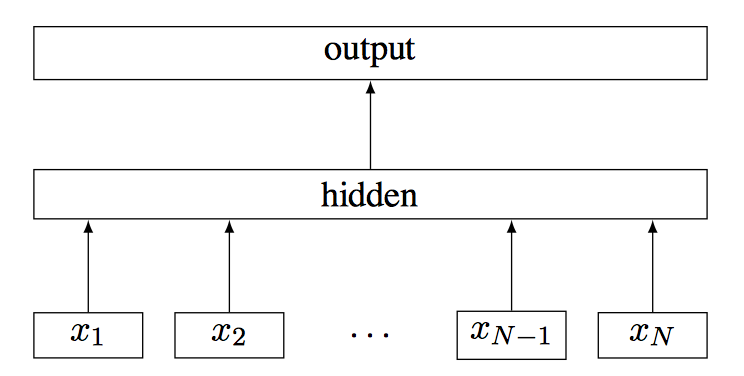
\includegraphics[width=.5\columnwidth]{fast_text}
\caption{\cite{joulin2016bag} Model architecture of \emph{fastText} for a sentence with $N$ n-gram features $x_1,\dots,x_N$. The features are embedded and averaged to form the hidden variable.}
\label{fig:fastText}
\end{figure}


\subsubsection{Convolutional Neural Network}
Convolutional Neural Networks are considered state of the art in many text classification problem.
This model is composed by a convolutional layer, followed by a global max pooling layer and two fully connected layers.

\subsubsection{KIM.}


\begin{figure}[h]
\footnotesize
\centering
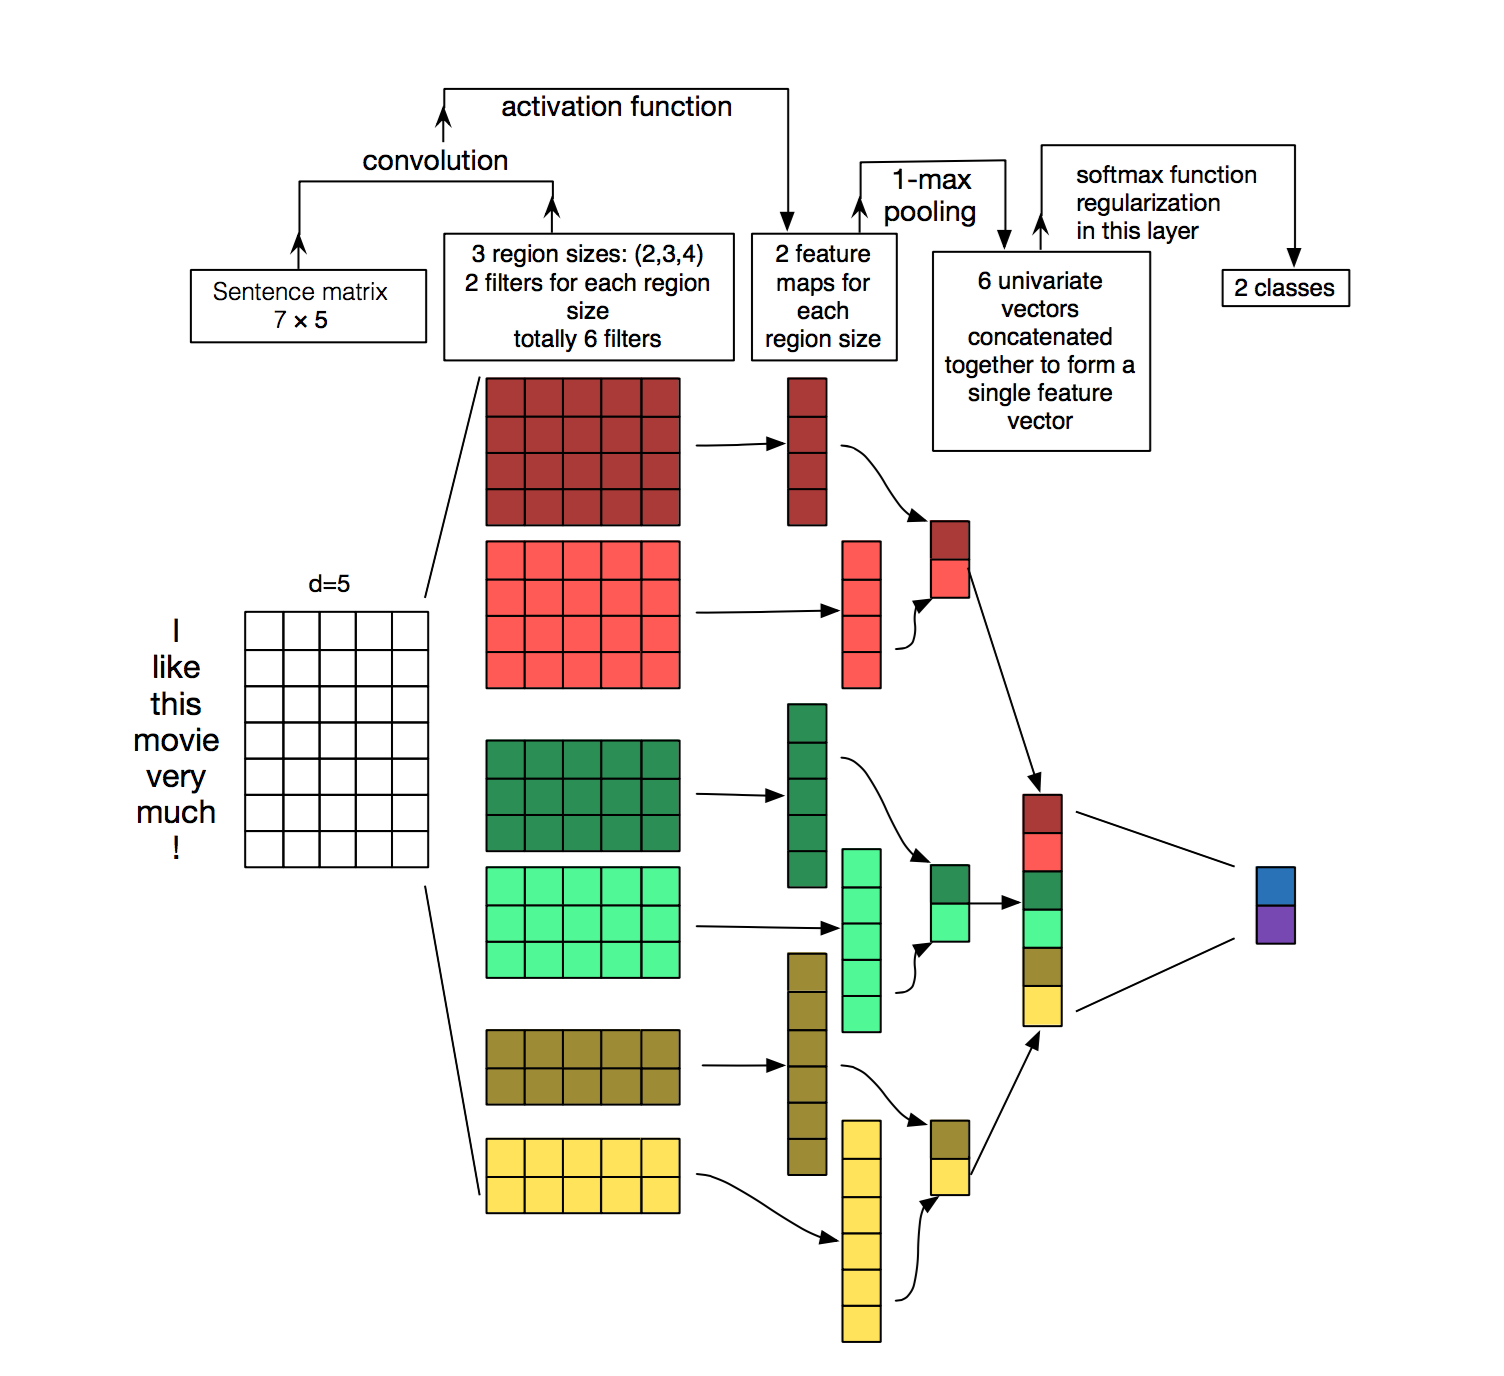
\includegraphics[width=.5\columnwidth]{kim_cnn}
\caption{\cite{zhang2015sensitivity} Illustration of a Convolutional Neural Network (CNN) architecture for sentence classification}
\label{fig:kim}
\end{figure}

This model is based on this paper \cite{kim2014convolutional}. It is based on different filter region size convolutions, followed by maxpooling layers.
All those outputs are concatenated to build sentence representation that is finally projected into a dense layer for the classification.
The intuition behind this model is that smaller filter region size should be able to capture short sentence patterns (similar to ngrams), while bigger sizes should capture sentence level features. We reached the best performance using [2, 3, 5, 7] as filter sizes.


\subsubsection{Long short-term memory}
LSTM is a type of Recurrent Neural Network (i.e. RNN) that is relatively insensitive to gap length, compared to others RNN, they are considered state of the art in machine translation.
In this model the classical embedding layer is followed by an LSTM layer with 128 units, terminated by a fully connected layer.
We also tried Bidirectional LSTM, 
% since they are bringing an improvement in different tasks, but they are performing worst on our use case.
To avoid overfitting we used droput and recurrent dropout, best results were obtained with a droput value of 0.4 and recurrent dropout value of 0.3.

